\chapter{Design} \label{cap:cap3}

\section{Persistance design}
<Identify the product whose software requirements are specified in this document, including the revision or release number. Describe the scope of the product that is covered by this SRS, particularly if this SRS describes only part of the system or a single subsystem.>

\section{MVC modeling}
<Describe any standards or typographical conventions that were followed when writing this SRS, such as fonts or highlighting that have special significance. For example, state whether priorities  for higher-level requirements are assumed to be inherited by detailed requirements, or whether every requirement statement is to have its own priority.>

\subsection{MVC structure}
\subsection{MVC behaviour}

\section{BCE Diagrams}
This paragraph illustrates the BCE pattern representing the architecture that we'll implement in order to develop the WeatherCal system. When identifying the elements for some scenario of system behavior, we can align each participating element with one of three key perspectives : Boundary, Control and Entity. \\This  pattern is a variation of the MVC pattern indeed we can consider mapping the Boundary with the MCV's View, the Control with the MCV's Controller and the Entity with the MVC's Model. Moreover the BCE pattern is not solely appropriate for dealing with user interfaces but it gives also to the controller a slightly different role to play.\\Let's take a deeper look in to the BCE pattern:\begin{itemize}
\item Entity: are objects representing system data and also they perform behavior organized around some cohesive amount of data.
\item Boundaries: are the objects that interface with system actors and most of the times they lay on periphery of a system. Some boundary elements will be "front-end" elements that accept input from outside the area under design and other elements will be "back-end" managing communication to supporting elements outside the system or subsystem.
\item Control: are the elements that mediate between boundaries and entities and control the flow of the interaction of the scenario. They manage the execution of commands coming from the boundary.
\subsection{Entity overview}
The diagram in~\ref{fig:entityovervie} illustrates an overview of all entities involved in our system and how they are related with each other.
 \begin{center}
 \begin{figure}[H]
    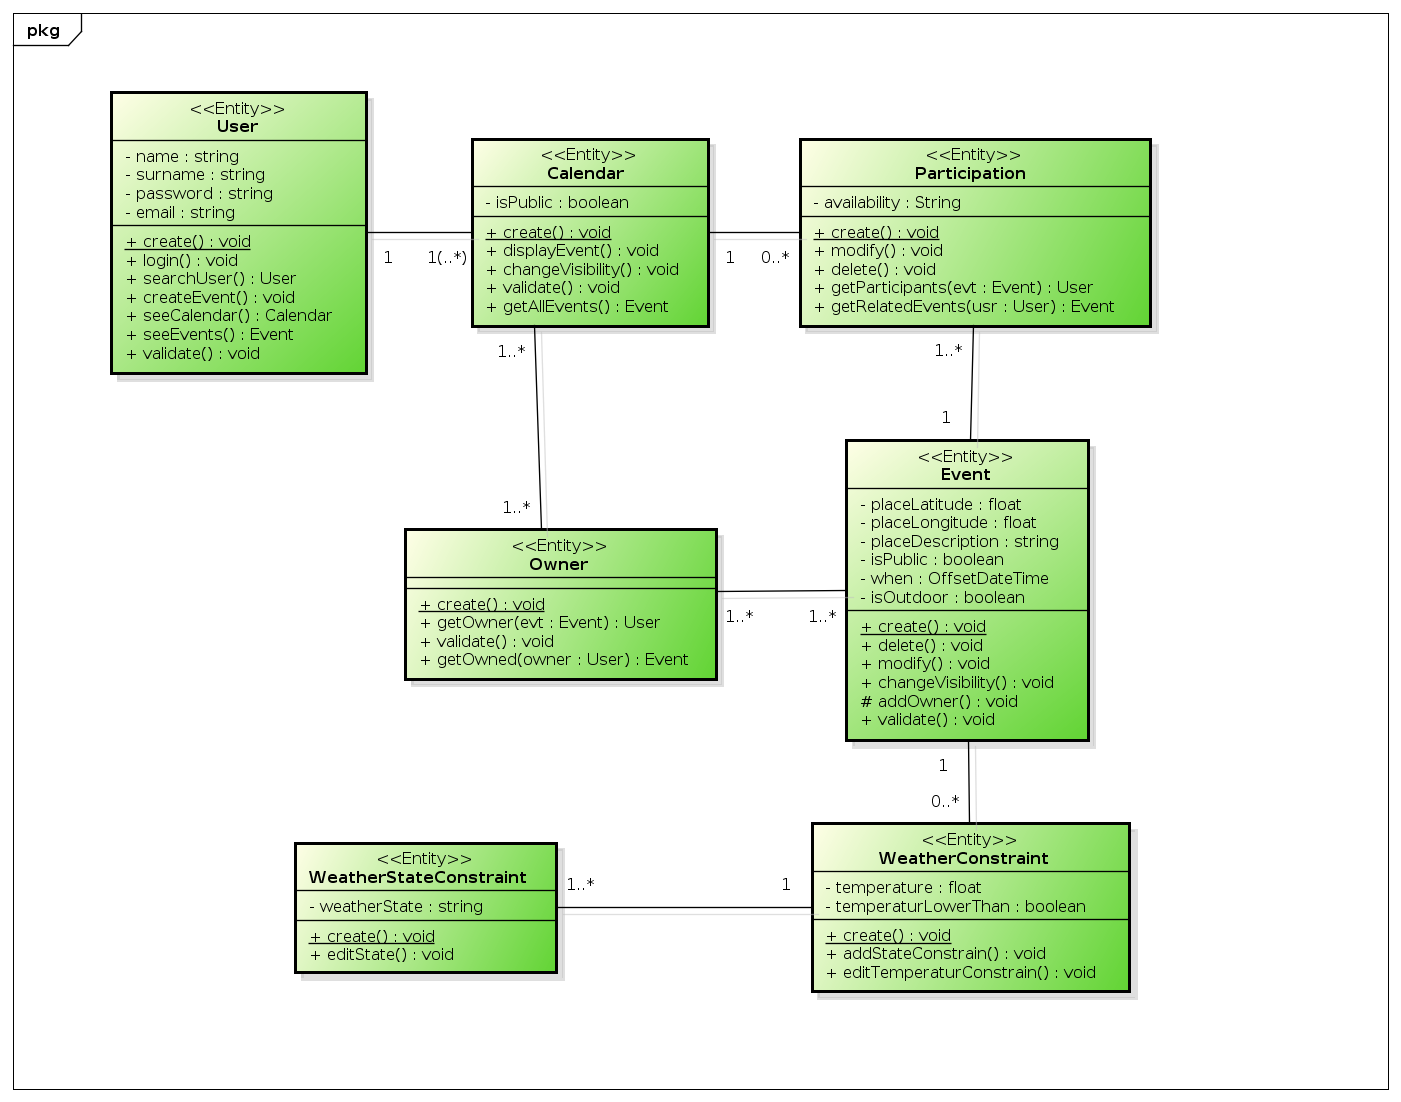
\includegraphics[width=1\textwidth]{../BCEDiagram/BCE/EntityOverview/Entity.png}
    \caption{Entities involved}
     \label{fig:entityovervie}
     \end{figure}
   \end{center}  


\subsection{Sign Up and Log In }
The diagram in~\ref{fig:logBCE} shows the flow of the system's behavior related to the registered user's login or to the anonymous user's signup. \\In these diagram there are only two entities who plays an active role:
\begin{enumerate}
\item Anonymous User: represents someone who is not signed in  to the system and can only reach the main page and sign up in to the platform
\item User: it's a registered user that can log in to the platform and gets to his UserPage
\end{enumerate}
There are two boundaries involved in this scenario: \begin{enumerate}
\item MainPage: it represents the index page of the system. The one in which a user can either log in or sign up to the platform.
\item UserPage: it stands for the page reach by the user after he logged in. It shows his calendar and all other tasks that the user can performs within it such as searches for a user, creates or modifies an event or checks for notification.
 \end{enumerate}
The controls who manage the flow of this scenario are two:\begin{enumerate}
\item SignUpManager: it's the control whose role is to handle the request of register a new user into the system. Whenever an anonymous user submits his information the SignUpManager verifies the correctness of these information and then create a new User and redirect him to the UserPage.
\item LoginManager: his task is to manage the log in of a registered user. It verifies that the credentials submitted by the user are the same provided in the system registration.   
\end{enumerate}
\begin{center}
 \begin{figure}[H]
    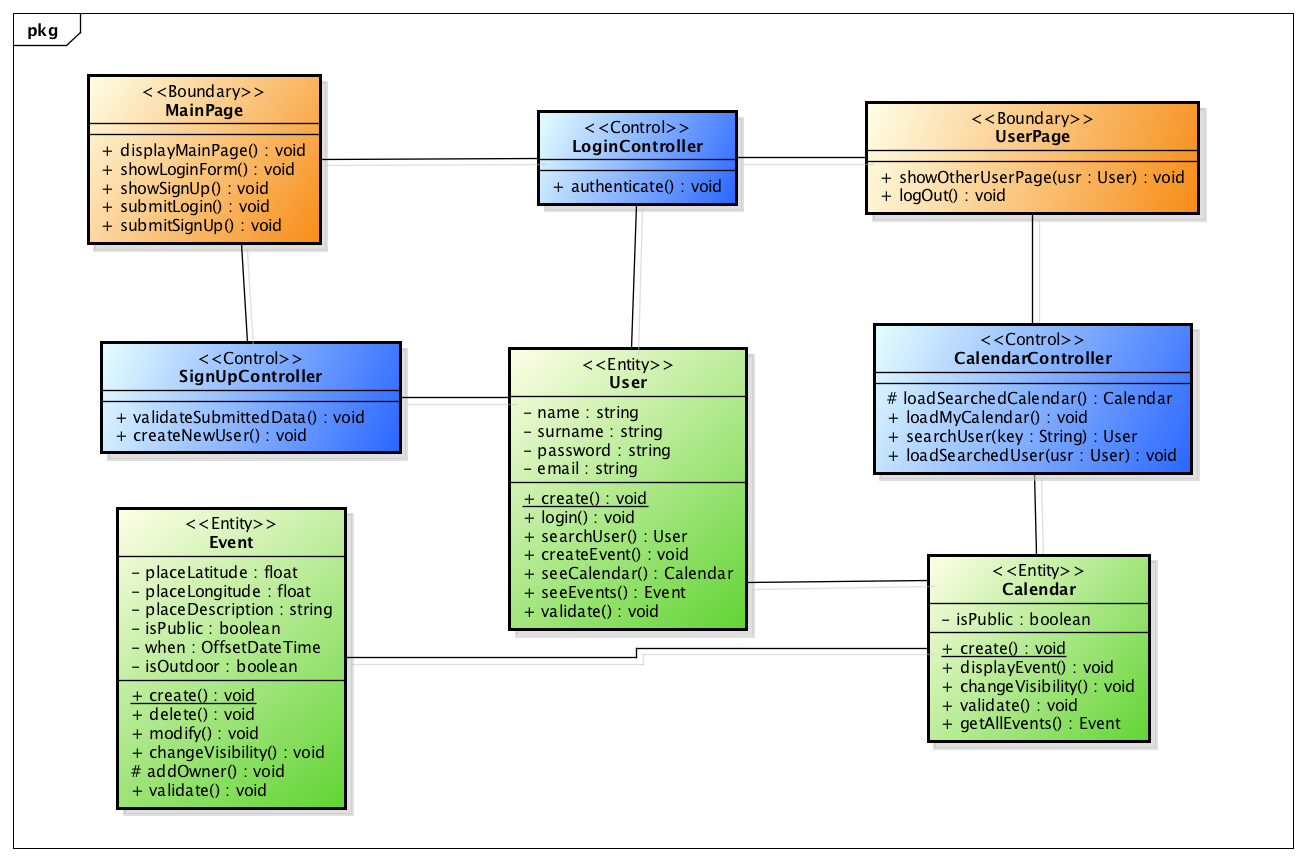
\includegraphics[width=1\textwidth]{../BCEDiagram/BCE/EntityOverview/LoginBCE.png}
    \caption{Sign Up and Log In}
     \label{fig:logBCE}
     \end{figure}
   \end{center}  
\end{itemize}

\subsection{Event creation or modification}
The diagram in~\ref{fig:editneweventBCE} illustrates the flow of the creation of the modification of an event. Naturally an user can perform   these action only if it's logged in to the system. The top side of the diagram it's related to the log in mechanism already seen in fig~\ref{fig:logBCE} while the bottom side represents the management of an event. 
\\In these diagram there are only two entities who plays an active role:
\begin{enumerate}
\item User: it's a registered user that can log in to the platform and gets to his UserPage.
\item Event: represents an event in the calendar. An user can be related to it in two different way, it could be a guest or it could be its owner. Depending on this relation it can perform different action. Modify or create it if it's an owner or change his participation if it's a guest.\end{enumerate}
There are two boundaries involved in this scenario: \begin{enumerate}
\item UserPage: it stands for the page reach by the user after he logged in. It shows his calendar and all other tasks that the user can performs within it such as searches for a user, creates or modifies an event or checks for notification.
\item NewModifyEventPage: is the page that a user uses to create or manage an event. It displays all the informations about the selected event such as the place, the date and the desired weather. More over gives to the owner of the event the capability to modify these data or to insert new informations in case the user is creating a new event.
 \end{enumerate}
The controls who manage the flow of this scenario are two:\begin{enumerate}
\item LoginManager: his task is to manage the log in of a registered user. It verifies that the credentials submitted by the user are the same provided in the system registration.   
\item EventController: this control has several duties many of which concerning the event creation or modification. It's able either to load the information regarding an existing event or to delete an event or to check the correctness of the submitted values for its attributes when the event is created.
\end{enumerate}



\begin{center}
 \begin{figure}[H]
    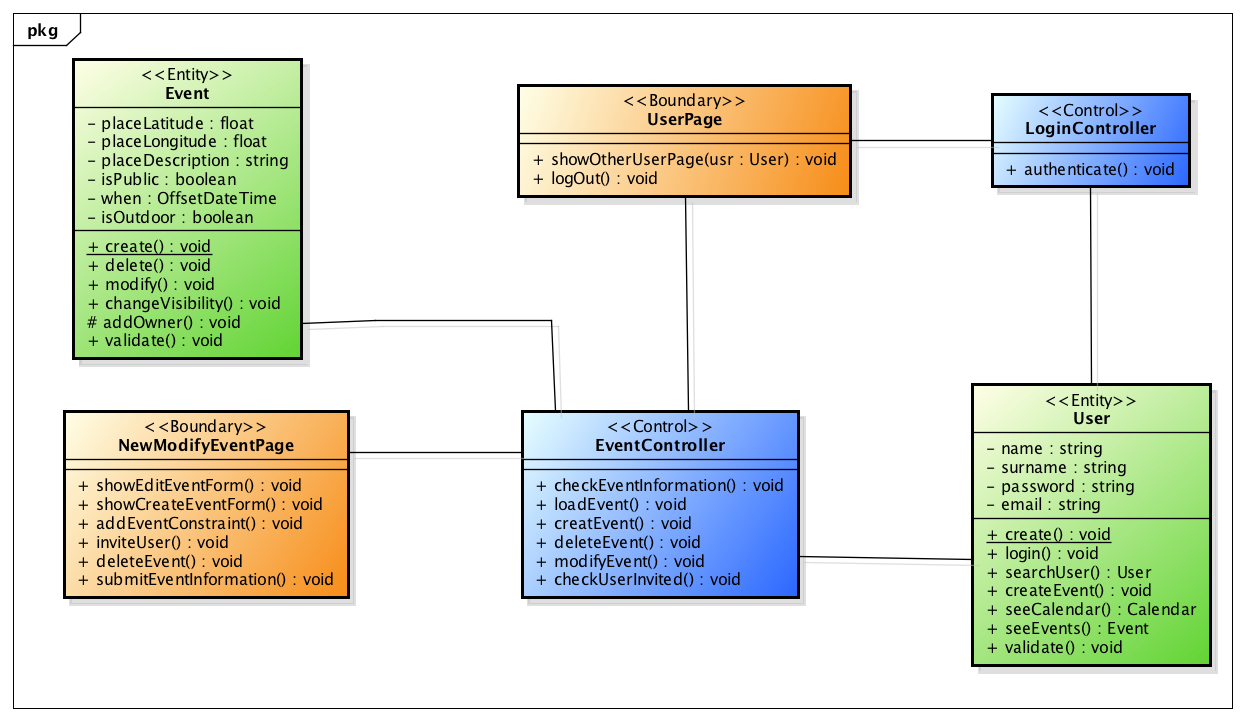
\includegraphics[width=1\textwidth]{../BCEDiagram/BCE/EntityOverview/EventManagementBCE.png}
    \caption{Create or modify an event}
     \label{fig:editneweventBCE}
     \end{figure}
   \end{center}  

